% Template:     Informe LaTeX
% Documento:    Archivo de ejemplo
% Versión:      7.0.0 (16/06/2020)
% Codificación: UTF-8
%
% Autor: Pablo Pizarro R.
%        Facultad de Ciencias Físicas y Matemáticas
%        Universidad de Chile
%        pablo@ppizarror.com
%
% Manual template: [https://latex.ppizarror.com/informe]
% Licencia MIT:    [https://opensource.org/licenses/MIT]

% ------------------------------------------------------------------------------
% NUEVA SECCIÓN
% ------------------------------------------------------------------------------
% Las secciones se inician con \section, si se quiere una sección sin número se
% pueden usar las funciones \sectionanum (sección sin número) o la función
% \sectionanumnoi para crear el mismo título sin numerar y sin aparecer en el índice
\section{Informes con \LaTeX}

	% SUB-SECCIÓN
	% Las sub-secciones se inician con \subsection, si se quiere una sub-sección
	% sin número se pueden usar las funciones \subsectionanum (nuevo subtítulo sin
	% numeración) o la función \subsectionanumnoi para crear el mismo subtítulo sin
	% numerar y sin aparecer en el índice
	\subsection{Una breve introducción}
		
		Este es un párrafo, puede contener múltiples \quotes{Expresiones} así como fórmulas o referencias\footnote{Las referencias se hacen utilizando la expresión \texttt{\textbackslash label}\{etiqueta\}.} como \eqref{eqn:identidad-imposible} ó (\ref{img:anexo-2}). A continuación se muestra un ejemplo de inserción de imágenes (como la Figura \ref{img:testimage}) con el comando \href{https://latex.ppizarror.com/informe.html#hlp-imagen}{\hreftext{\textbackslash insertimage}}:

		% Esta instrucción, añadida en la v6.5.5 permite cambiar el título de cada
		% objeto en el índice de cada objeto. Este título es solo válido hasta el
		% primer objeto que lo llame, luego este se reestablecerá. Por mientras solo
		% se ofrece compatibilidad para las funciones de imágenes. Los entornos como
		% images o sourcecode aún no tienen compatibilidad
		\setindexcaption{Título de la imagen en el índice.}
		
		% Para insertar una imagen se puede usar la función \insertimage la cual
		% toma un primer parámetro opcional para definir una etiqueta (dentro de
		% los corchetes), luego toma la dirección de la imagen, sus parámetros
		% (en este caso se definió la escala de 0.15) y una leyenda opcional
		\insertimage[\label{img:testimage}]{ejemplos/test-image.png}{scale=0.15}{Where are you? de \quotes{Internet}.}

		A continuación\footnote{Como se puede observar las funciones \texttt{\textbackslash insert...} añaden un párrafo automáticamente.} se muestra un ejemplo de inserción de ecuaciones simples con el comando \href{https://latex.ppizarror.com/informe.html#hlp-formulae}{\hreftext{\textbackslash insertequation}}:

		% Se inserta una ecuación, el primer parámetro entre [] es opcional
		% (permite identificar con una etiqueta para poder referenciarlo después
		% con \ref), seguido de aquello se escribe la ecuación en modo bruto sin signos $
		\insertequation[\label{eqn:identidad-imposible}]{\pow{a}{k}=\pow{b}{k}+\pow{c}{k} \quad \forall k>2}

		% Notar que no se requiere añadir un salto de línea después de insertar una imagen
		Este template ha sido diseñado para que sea completamente compatible con editores \LaTeX\ para escritorio y de manera online \scite{overleaf}. La compilación es realizada siempre usando las últimas versiones de las librerías, además se incluyen los parches oficiales para corregir eventuales \textit{warnings}.

		% Los párrafos se pueden añadir con \newp, esta función se hizo para evitar
		% errores y warnings por parte del compilador de LaTeX
		\newp Este es un nuevo párrafo insertado con el comando \href{https://latex.ppizarror.com/informe.html#hlp-parrafo}{\hreftext{\textbackslash newp}}. Si no te gustan los comandos \texttt{\textbackslash newp}, \texttt{\textbackslash newpar} o \texttt{\textbackslash newparnl} simplemente puedes usar los salto de línea convencionales acompañado de \texttt{\textbackslash par}.

	% SUB-SECCIÓN
	\subsection{Añadiendo tablas}

		También puedes usar tablas, ¡Crearlas es muy fácil!. Puedes usar el plugin \href{https://www.ctan.org/tex-archive/support/excel2latex/}{Excel2Latex} \cite{excel2latex} de Excel para convertir las tablas a \LaTeX\ o bien utilizar el \quotes{creador de tablas online} \cite{tablesgenerator}.

		% Tabla generada con el plugin Excel2Latex
		\begin{table}[htbp]
			\centering
			\caption{Ejemplo de tablas.}
			\begin{tabular}{ccc}
				\hline
				\textbf{Columna 1} & \textbf{Columna 2} & \textbf{Columna 3} \bigstrut\\
				\hline
				$\omega$ & $\nu$ & $\delta$ \bigstrut[t]\\
				$\Phi$ & $\Theta$ & $\varSigma$ \\
				$\xi$ & $\kappa$ & $\varpi$ \bigstrut[b] \\
				\hline
			\end{tabular}
			\label{tab:tabla-1}
		\end{table}


% ------------------------------------------------------------------------------
% NUEVA SECCIÓN
% ------------------------------------------------------------------------------
\newpage
\section{Aquí un nuevo tema}

	% SUB-SECCIÓN
	\subsection{Haciendo informes como un profesional}

		% Se inserta una imagen flotante en la izquierda del documento con
		% \insertimageleft, al igual que las demás funciones, el primer parámetro
		% es opcional, luego viene la ubicación de la imagen, seguido de la escala
		% (un 30% del ancho de página) y por último su leyenda. Para insertar una
		% imagen flotante en la derecha se utiliza \insertimageright usando los
		% mismos parámetros
		\insertimageleft[\label{img:imagen-izquierda}]{ejemplos/test-image-wrap}{0.3}{Apolo flotando a la izquierda.}
		
		~ \lipsum[1]

		% Párrafos de ejemplo
		\newp \lipsum[115]

		% Agrega una ecuación en el índice
		\insertindexequation[\label{eqn:formulasinsentido}]{\int_{a}^{b} f(x) \dd{x} = \fracnpartial{f(x)}{x}{\eta} \cdotp \textstyle \sum_{x=a}^{b} f(x)\cancelto{1+\frac{\epsilon}{k}}{\bigp{1+\Delta x}}}{Ecuación sin sentido.}

		% Inserta una definición, compatibilidad con otros templates
		\begin{defn}[ver \cite{templateinforme}]
			Definición definitiva
			$$\frac{d}{dx}\int_a^xf(y)dy=f(x)$$
		\end{defn}

		% Aquí no es necesario usar \newp dado que todas las funciones \insert...
		% añaden un párrafo nuevo por defecto
		\lipsum[115]
		\newp \lipsum[116]

	% Inserta un subtítulo sin número
	\subsection{Otros párrafos más normales}

		% Párrafos
		\lipsum[7]
		\newp \lipsum[2]

		% Se inserta una ecuación larga con el entorno gathered (1 solo número de ecuación)
		\insertgathered[\label{eqn:eqn-larga}]{
			\lpow{\Lambda}{f} = \frac{L\cdot f}{W} \cdot \frac{\pow{\lpow{Q}{e}}{2}}{8 \pow{\pi}{2} \pow{W}{4} g} + \sum_{i=1}^{l} \frac{f \cdot \bigp{M - d}}{l \cdot W} \cdot \frac{\pow{\bigp{\lpow{Q}{e}- i\cdot Q}}{2}}{8 \pow{\pi}{2} \pow{W}{4} g}\\
			Q_e = 2.5Q \cdot \int_{0}^{e} V(x) \dd{x} + \aasin{\biggp{1+\frac{1}{1-e}}}
		}

		% Nuevo párrafo
		\lipsum[4]

		% Se inserta un multicols, con esto se pueden escribir párrafos en varias columnas
		\begin{multicols}{2}

			% Párrafo 1
			\lipsum[4-5]

			% Ecuación encerrada en una caja
			\insertequation[]{ \boxed{f(x) = \fracdpartial{u}{t}} }
			
			% Párrafo 2
			\lipsum[6-7]
			
			% Inserta una imagen simple
			\insertimage{ejemplos/test-image-wrap}{width=4cm}{Imagen dentro de párrafo.}

			% Párrafo 2 del multicols
			\lipsum[1-2]
			
			\begin{figure*}[b!]
				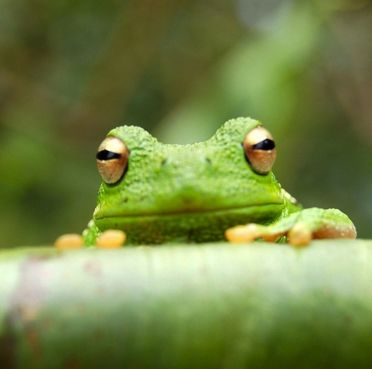
\includegraphics[width=5cm,height=4cm]{ejemplos/test-image-wrap}
				\caption{This is a tiger.}
			\end{figure*}
		
			\lipsum[1-20]

		\end{multicols}

	% SUB-SECCIÓN
	\subsection{Ejemplos de inserción de código fuente}

		% A continuación se crea una función auxiliar, esta es una herramienta
		% extremadamente importante y muy útil. Esta función de ejemplo toma dos
		% parámetros, uno es el lenguaje del código fuente, el segundo el
		% identificador en el manual
		\newcommand{\insertsrcmanual}[2]{\href{https://latex.ppizarror.com/informe.html?srctype=#1\#hlp-srccode}{#2}}

		El template permite la inserción de los siguientes lenguajes de programación de forma nativa: \insertsrcmanual{assemblerx64}{Assembler x64}, \insertsrcmanual{assemblerx86}{Assembler x86[masm]},  \insertsrcmanual{bash}{Bash}, \insertsrcmanual{c}{C}, \insertsrcmanual{cpp}{C++}, \insertsrcmanual{csharp}{C\#}, \insertsrcmanual{css}{CSS}, \insertsrcmanual{csv}{CSV}, \insertsrcmanual{cuda}{CUDA}, \insertsrcmanual{docker}{DOCKER}, \insertsrcmanual{fortran}{Fortran}, \insertsrcmanual{glsl}{GLSL}, \insertsrcmanual{haskell}{Haskell}, \insertsrcmanual{html5}{HTML5}, \insertsrcmanual{ini}{INI}, \insertsrcmanual{java}{Java}, \insertsrcmanual{js}{Javascript}, \insertsrcmanual{json}{JSON}, \insertsrcmanual{kotlin}{Kotlin}, \insertsrcmanual{latex}{LaTeX}, \insertsrcmanual{lisp}{Lisp}, \insertsrcmanual{lua}{Lua}, \insertsrcmanual{maple}{Maple}, \insertsrcmanual{matlab}{Matlab}, \insertsrcmanual{octave}{Octave}, \insertsrcmanual{opencl}{OpenCL}, \insertsrcmanual{opensees}{OpenSees}, \insertsrcmanual{pascal}{Pascal}, \insertsrcmanual{perl}{Perl}, \insertsrcmanual{php}{PHP}, \insertsrcmanual{plaintext}{Texto plano}, \insertsrcmanual{pseudocode}{Pseudocódigo}, \insertsrcmanual{python}{Python}, \insertsrcmanual{r}{R}, \insertsrcmanual{ruby}{Ruby}, \insertsrcmanual{scala}{Scala}, \insertsrcmanual{scheme}{Scheme}, \insertsrcmanual{sql}{SQL}, \insertsrcmanual{tcl}{TCL}, \insertsrcmanual{vbscript}{VBScript}, \insertsrcmanual{verilog}{Verilog}, \insertsrcmanual{vhdl}{VHDL} y \insertsrcmanual{xml}{XML}. \\
		
		Para insertar un código fuente se debe usar el entorno \texttt{sourcecode}, o el entorno \texttt{sourcecodep} si es que se quiere utilizar parámetros adicionales. A continuación se presenta un ejemplo de inserción de código fuente en Python (Código \ref{codigo-python}), Java y Matlab:

% Se define el lenguaje del código. Cuidado: Los códigos en LaTeX son sensibles
% a las tabulaciones y espacios en blanco
\begin{sourcecode}[\label{codigo-python}]{python}{Ejemplo en Python.}
import numpy as np

def incmatrix(genl1, genl2):
	m = len(genl1)
	n = len(genl2)
	M = None # Comentario 1
	VT = np.zeros((n*m, 1), int) # Comentario 2
\end{sourcecode}

\begin{sourcecode}[]{java}{Ejemplo en Java.}
import java.io.IOException;
import javax.servlet.*;

// Hola mundo
public class Hola extends GenericServlet {
	public void service(ServletRequest request, ServletResponse response)
	throws ServletException, IOException{
		response.setContentType("text/html");
		PrintWriter pw = response.getWriter();
		pw.println("Hola, mundo!");
	}
}
\end{sourcecode}

\begin{sourcecode}{matlab}{Ejemplo en Matlab.}
% Se crea gráfico
f = figure(1); hold on; movegui(f, 'center');
xlabel('td/Tn'); ylabel('FAD=Umax/Uf0');
title('Espectro de pulso de desplazamiento');

for j = 1:length(BETA)
	fad = ones(1, NDATOS); % Arreglo para el FAD
	for i = 1:NDATOS
		[t, u_t, ~, ~] = main(BETA(j), r(i), M, K, F0, 0);
		fad(i) = max(abs(u_t)) / uf0;
	end
end
\end{sourcecode}

	% SUB-SECCIÓN
	\subsection{Añadir múltiples imágenes}

	El template ofrece el entorno \href{https://latex.ppizarror.com/informe#hlp-images}{\hreftext{images}} que permite insertar múltiples imágenes de una manera muy sencilla. Para crear imágenes múltiples se deben usar las siguientes instrucciones:

\begin{sourcecode}{latex}{}
\begin{images}[\label{imagenmultiple}]{Ejemplo de imagen múltiple.}
	\addimage{ejemplos/test-image}{width=6.5cm}{Ciudad.}
	\addimage{ejemplos/test-image-wrap}{width=5cm}{Apolo.}
	\imagesnewline
	\addimage{ejemplos/test-image}{width=12.5cm}{Ciudad más grande.}
\end{images}
\end{sourcecode}

	Obteniendo así:

	\begin{images}{Ejemplo de imagen múltiple.}
		\addimage{ejemplos/test-image}{width=6.5cm}{Ciudad.}
		\addimage{ejemplos/test-image-wrap}{width=5cm}{Apolo.}
		\imagesnewline
		\addimage{ejemplos/test-image}{width=12.5cm}{Ciudad más grande.}
	\end{images}


% ------------------------------------------------------------------------------
% NUEVA SECCIÓN
% ------------------------------------------------------------------------------
% Inserta una sección sin número
\sectionanum{Más ejemplos}

	% Inserta un subtítulo sin número
	\subsectionanum{Listas y Enumeraciones}

		Hacer listas enumeradas con \LaTeX\ es muy fácil con el template,\footnote{También puedes revisar el manual de las enumeraciones en \url{http://www.texnia.com/archive/enumitem.pdf}.} para ello debes usar el comando \texttt{\textbackslash begin\{enumerate\}}, cada elemento comienza por \texttt{\textbackslash item}, resultando así:

		\begin{enumerate}
			\item Grecia
			\item Abracadabra
			\item Manzanas
		\end{enumerate}

		También se puede cambiar el tipo de enumeración, se pueden usar letras, números romanos, entre otros. Esto se logra cambiando el \textbf{label} del objeto \texttt{enumerate}. A continuación se muestra un ejemplo usando letras con el estilo \texttt{\textbackslash alph},\footnote{Con \texttt{\textbackslash Alph} las letras aparecen en mayúscula.} números romanos con \texttt{\textbackslash roman}\footnote{Con \texttt{\textbackslash Roman} los números romanos salen en mayúscula.} o números griegos con \texttt{\textbackslash greek}:\footnote{Una característica propia del template, con \texttt{\textbackslash Greek} las letras griegas están escritas en mayúscula.}

		\begin{multicols}{3}
			\begin{enumeratebf}[label=\alph*) ] % Fuente en negrita
				\item Peras
				\item Manzanas
				\item Naranjas
			\end{enumeratebf}

			\begin{enumerate}[label=\greek*) ]
				\item Matemáticas
				\item Lenguaje
				\item Filosofía
			\end{enumerate}

			\begin{enumerate}[label=\roman*) ]
				\item Rojo
				\item Café
				\item Morado
			\end{enumerate}
		\end{multicols}

		Para hacer listas sin numerar con \LaTeX\ hay que usar el comando \texttt{\textbackslash begin\{itemize\}}, cada elemento empieza por \texttt{\textbackslash item}, resultando:

		\begin{multicols}{3}
			\begin{itemize}[label={--}]
				\item Peras
				\item Manzanas
				\item Naranjas
			\end{itemize}

			\begin{enumerate}[label={*}]
				\item Rojo
				\item Café
				\item Morado
			\end{enumerate}

			\begin{itemize}
				\item Árboles
				\item Pasto
				\item Flores
			\end{itemize}
		\end{multicols}

	% Inserta un subtítulo sin número
	\subsectionanum{Otros}

		Recuerda revisar el manual de todas las funciones y configuraciones de este template visitando el siguiente link: \url{https://latex.ppizarror.com/informe}. Si necesitas una ayuda muy específica sobre el template, o si tienes alguna sugerencia, me puedes enviar un correo a \insertemail{pablo@ppizarror.com}.


% ------------------------------------------------------------------------------
% REFERENCIAS (ESTILO BIBTEX), revisar configuración \stylecitereferences
% ------------------------------------------------------------------------------
\newpage % Salto de página
\begin{references}
	\bibitem{templateinforme}
	Template Informe en \LaTeX.
	\textit{¡Revisa el manual online de este template!} \\
	\url{https://latex.ppizarror.com/informe}

	\bibitem{excel2latex}
	Excel2Latex.
	\textit{Importa de forma sencilla tus tablas de Excel a \LaTeX.} \\
	\url{https://www.ctan.org/tex-archive/support/excel2latex/}

	\bibitem{overleaf}
	Overleaf.
	\textit{Uno de los mejores editores online para \LaTeX, renovado con su versión 2.0.} \\
	\href{https://es.overleaf.com}{\hreftext{https://es.overleaf.com/}}
	
	\bibitem{tablesgenerator}
	Tables Generator.
	\textit{Creador de tablas online para \LaTeX.}\\
	\url{https://www.tablesgenerator.com}
\end{references}


% ------------------------------------------------------------------------------
% ANEXO
% ------------------------------------------------------------------------------
\newpage
\begin{anexo}

\section{Cálculos realizados}

	\subsection{Metodología}
		\lipsum[1] \eqref{eqn:identidad-imposible}

		% Imagen, se numerará automáticamente con la letra del anexo según
		% la configuración \appendixindepobjnum
		\insertimage[\label{img:anexo-2}]{ejemplos/test-image.png}{scale=0.2}{Imagen en anexo.}

	\subsection{Resultados}
		\lipsum[10]

		% Tablas
		\enabletablerowcolor[2] % Activa el color de celda
		\begin{table}[htbp]
			\centering
			\caption{Tabla de cálculo.}
			\begin{tabular}{ccc}
				\hline
				\textbf{Elemento} & $\epsilon_i$ & \boldmath{}\textbf{Valor}\unboldmath{} \bigstrut\\
				\hline
				A     & 10    & 3,14$\pi$ \bigstrut[t]\\
				B     & 20    & 6 \\
				C     & 30    & 7 \\
				D     & 150    & 10 \\
				E     & 0    & 0 \\
				\hline
				\end{tabular}
			\label{tab:anexo-1}
		\end{table}
		\disabletablerowcolor % Desactiva el color de celda

\newpage
\section{Más cálculos}

	% Párrafo
	\lipsum[1]

	% Nuevo párrafo con identación
	\newp \lipsum[4]

	% Tabla de encuestas
	\begin{table}[htbp]
		\centering
		\caption{Resultados encuesta.}
		\begin{tabular}{ccc}
			\hline
			\textbf{Herramienta} & \textbf{Nota} & \textbf{Recomendado} \bigstrut\\
			\hline
			\LaTeX & 100\% & Si $\checkmark$ \\
			Microsoft Word \textsuperscript{\textregistered} & 0\% & No $\frownie$\\
			\hline
		\end{tabular}
		\label{tab:anexo-2}
	\end{table}

	\lipsum[6]
	
	\insertindexequation{a=b+c}{Ecuación muy difícil}

\end{anexo}